\documentclass[12pt]{article}
	\usepackage[english]{babel}
	\usepackage[utf8x]{inputenc}
	\usepackage{amsmath}
	\usepackage{graphicx}
	\usepackage[colorinlistoftodos]{todonotes}
	
	\begin{document}
	
	\begin{titlepage}
	
	\newcommand{\HRule}{\rule{\linewidth}{0.5mm}} % Defines a new command for the horizontal lines, change thickness here
	
	\center % Center everything on the page
	 
	%----------------------------------------------------------------------------------------
	%	HEADING SECTIONS
	%----------------------------------------------------------------------------------------
	
	\textsc{\LARGE Testing Policy}\\[0.5cm] % Name of your university/college
	\textsc{\Large Team Hackermen}\\[0.5cm] % Major heading such as course name
	
	
	%----------------------------------------------------------------------------------------
	%	TITLE SECTION
	%----------------------------------------------------------------------------------------
	
	\HRule \\[0.4cm]
	{ \huge \bfseries TicketSalad}\\[0.4cm] % Title of your document
	\HRule \\[1.5cm]
	 
	%----------------------------------------------------------------------------------------
	%	AUTHOR SECTION
	%----------------------------------------------------------------------------------------
	
	\begin{minipage}{0.4\textwidth}
	\begin{flushleft} \large
	\emph{Team Members:}\\
	John \textsc{Smith} \\% Your name
	Thato \textsc{Mothusi}\\
	Jarryd \textsc{Baillie}\\
	Brandon \textsc{Texeira}\\
	Thomas \textsc{Honiball}\\
	Tristan \textsc{Joseph}\\
	\end{flushleft}
	\end{minipage}
	~
	\begin{minipage}{0.4\textwidth}
	\begin{flushright} \large
	\emph{Client:} \\
	Tribus Digita % Supervisor's Name
	\end{flushright}
	\end{minipage}\\[2cm]
	
	% If you don't want a supervisor, uncomment the two lines below and remove the section above
	%\Large \emph{Author:}\\
	%John \textsc{Smith}\\[3cm] % Your name
	
	
	%----------------------------------------------------------------------------------------
	%	LOGO SECTION
	%----------------------------------------------------------------------------------------
	
	
\includegraphics{logo.png}\\[1cm] % Include a department/university logo - this will require the graphicx package
	 
	%----------------------------------------------------------------------------------------
	
	\vfill % Fill the rest of the page with whitespace
	
	\end{titlepage}
	
	\section{Testing Processes}
	Since we are adopting scrum methodology and it does not say much about the testing process, we decided to adopt a waterfall approach within our sprint.Our sprints usually last 2 weeks and within those two weeks we develop certain features of the system and once those features are completed, we then write tests for those features we developed. So we are essentially using a white-box testing method whereby we first write code for the system and then write the test cases once we have knowledge of the source code.
	
	\subsection{Functional Requirements Tested}
	\begin{itemize}
		\item A user is able to register
		\item A user is able to login
		\item A user is able to claim on an event
		\item A user is notified if they won the ticket
		\item A user is able to view their profile
		\item A user is able to edit their details
		\item A user is able to search for events
		\item A user is able to logout
	\end{itemize}
	
	\subsection{Non-Functional Requirements Tested}
	\begin{itemize}
		\item The users password is encrypted
		\item The system responds in no more than 3 seconds
		\item The system displays the correct error messages
		\begin{itemize}
			\item Invalid username entered
			\item Invalid password entered
			\item Required data not entered
		\end{itemize}
	\end{itemize}
	
	\section{Testing Tools}
	Nightwatch is an automated testing framework for web applications and websites, written in Node.js and using the W3C Web-driver API (formerly Selenium Web-driver).Nightwatch relies on "nightwatch.json" as the configuration file to run test files, this json file is placed on the project's root directory. The json file allows for the specification of configuration settings like test environments, test file paths, and selenium specific settings.The reason we chose to use nightwatch is beacuse it has a simple but powerful syntax which enables us to write tests very quickly, using languages like javascript and CSS or Xpath selectors. It also has a built in command-line test runner which can run tests either sequentially or in parallel. Lastly nightwatch allows for flexibility, what this means is that there is a flexible command and assertion framework which makes it easy to extend to implement our application specific commands and assertions.
	
	
	\section{Test Cases}
	Our test cases are located on the master branch in a folder called Testing.Below is a tree structure of where our test cases are located on git.
	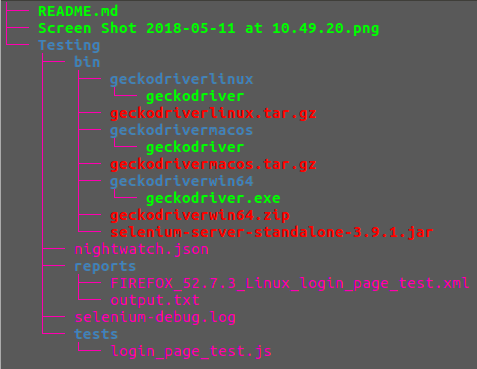
\includegraphics[width=0.8\linewidth, height=8cm]{tree.png}
	
	\section{History}
	
	
	
	
	
	
	
	
	
	\end{document}
	